\documentclass{rapport}
\usepackage{lipsum}
\usepackage{gensymb}
\usepackage{float}
\usepackage{minted}

\usepackage{graphicx} % Required for inserting images
\title{Lab 6 Report} %title of the file
\begin{document}

%----------- Report information ---------

\logo{logos/chico.png}
\uni{\textbf{California State Univeristy, Chico}}
\ttitle{Assignment 3 - Report} %title of the file
\subject{CSCI 612: Applied Computer Vision} % Subject name
\topic{Assignment 3} % Topic name

\professor{\textsc{Dr Sam Seiwart}} % information related to the professor

\students{
          \textsc{Akshay Aralikatti}} % information related to the students

%----------- Init -------------------
        
\buildmargins % display margins
\buildcover % create the front cover of the document
\toc % creates the table of contents

\section{Introduction}
The report shows the two ways to implement a program in C++ that reads a text file from standard input and compiles an alphabetical index of which words appear on which lines using Ternary Search Tree (TST) and Trie.

\section{Time and Space Complexity using Trie}

\begin{center}
\begin{tabular}{|c|c|c|}
\hline
\textbf{Function} & \textbf{Time Complexity} & \textbf{Space Complexity} \\
\hline
\texttt{insert} & \(O(k)\) & \(O(k)\) \\
\hline
\texttt{print} & \(O(n)\) & \(O(h)\) \\
\hline
\texttt{\_\_insert} & \(O(k)\) & \(O(k)\) \\
\hline
\texttt{\_\_print} & \(O(n)\) & \(O(h)\) \\
\hline
\texttt{\_\_delete} & \(O(n)\) & \(O(h)\) \\
\hline
\texttt{convertToWords} & \(O(m)\) & \(O(m)\) \\
\hline
\end{tabular}
\end{center}
Where:
\begin{itemize}
    \item \(k\): Average length of the word.
    \item \(m\): Length of the input string.
    \item \(n\): Total number of nodes in the Trie.
    \item \(h\): Height of the Trie (maximum word length).
\end{itemize}
\section{Valgrind output for the Trie implementation}
\begin{figure}[H]
    \centering
    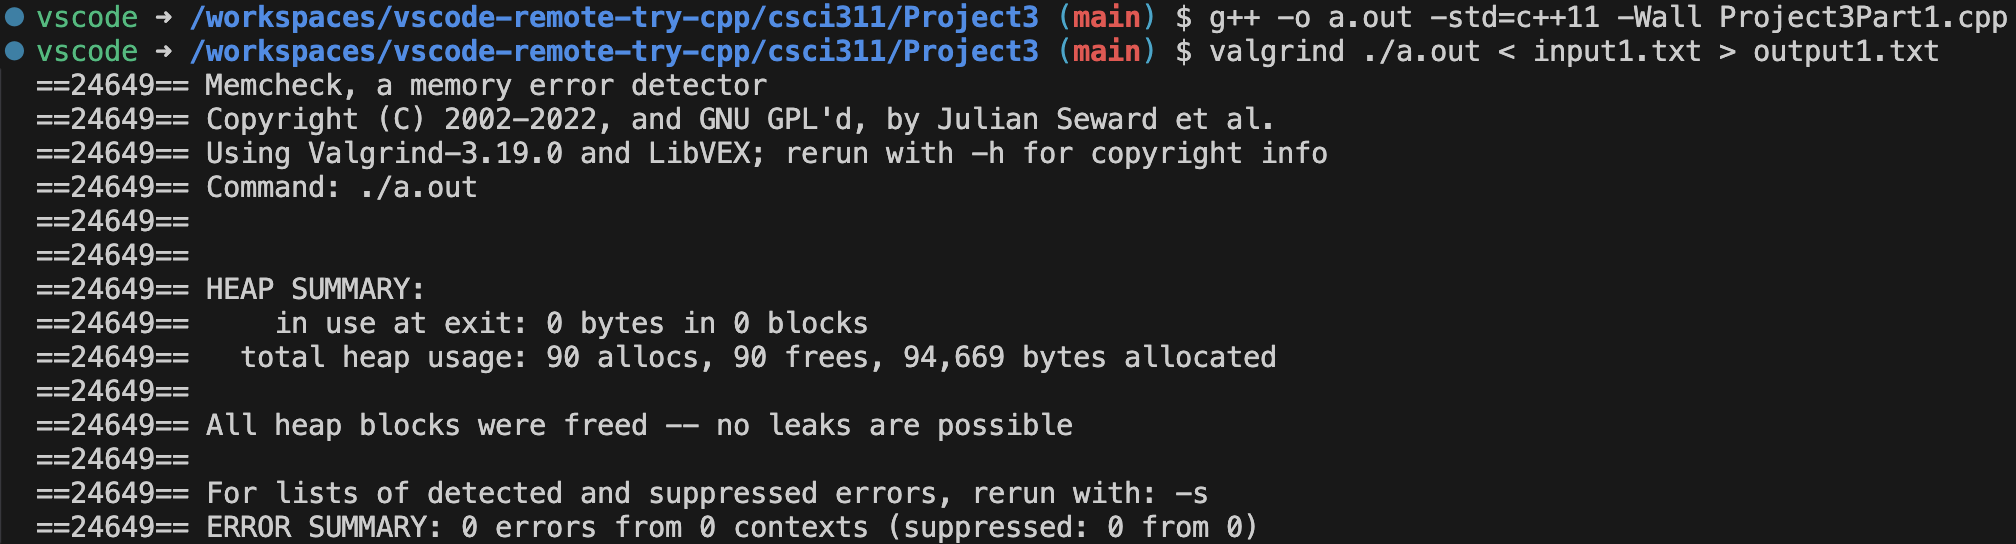
\includegraphics[width=1\textwidth]{v1.png}
    \caption{Valgrind results of Trie}
    \label{fig:trie_valgrind}
\end{figure}

\section{Recurrence Analysis for Trie}
\subsection{Print Function (print)}
\[
T(n) = T(n - 1) + O(1)
\]
Using substitution:
\[
T(n) = O(n)
\]
\textbf{Explanation:} The \texttt{print} function visits each node in the Trie exactly once.

\subsection{Delete Function (delete)}
\[
T(n) = T(n - 1) + O(1)
\]
Using substitution:
\[
T(n) = O(n)
\]
\textbf{Explanation:} The \texttt{delete} function visits each node in the Trie exactly once.



\section{Time and Space Complexity using Ternary Search Tree (TST)}

\begin{center}
\begin{tabular}{|c|c|c|}
\hline
\textbf{Function} & \textbf{Time Complexity} & \textbf{Space Complexity} \\
\hline
\texttt{insert} & \(O(k)\) & \(O(k)\) \\
\hline
\texttt{print} & \(O(n)\) & \(O(h)\) \\
\hline
\texttt{\_\_insert} & \(O(k)\) & \(O(k)\) \\
\hline
\texttt{\_\_print} & \(O(n)\) & \(O(h)\) \\
\hline
\texttt{convertToWords} & \(O(m)\) & \(O(m)\) \\
\hline
\texttt{\_\_delete} & \(O(n)\) & \(O(h)\) \\
\hline
\end{tabular}
\end{center}

Where:
\begin{itemize}
    \item \(k\): Average length of a word.
    \item \(w\): Total number of words in the input.
    \item \(m\): Length of the input string.
    \item \(n\): Total number of nodes in the TST.
    \item \(h\): Height of the TST.
    \item \(d\): Size of the alphabet (26 for lowercase English letters).
\end{itemize}
\section{Valgrind output for the TST implementation}
\begin{figure}[H]
    \centering
    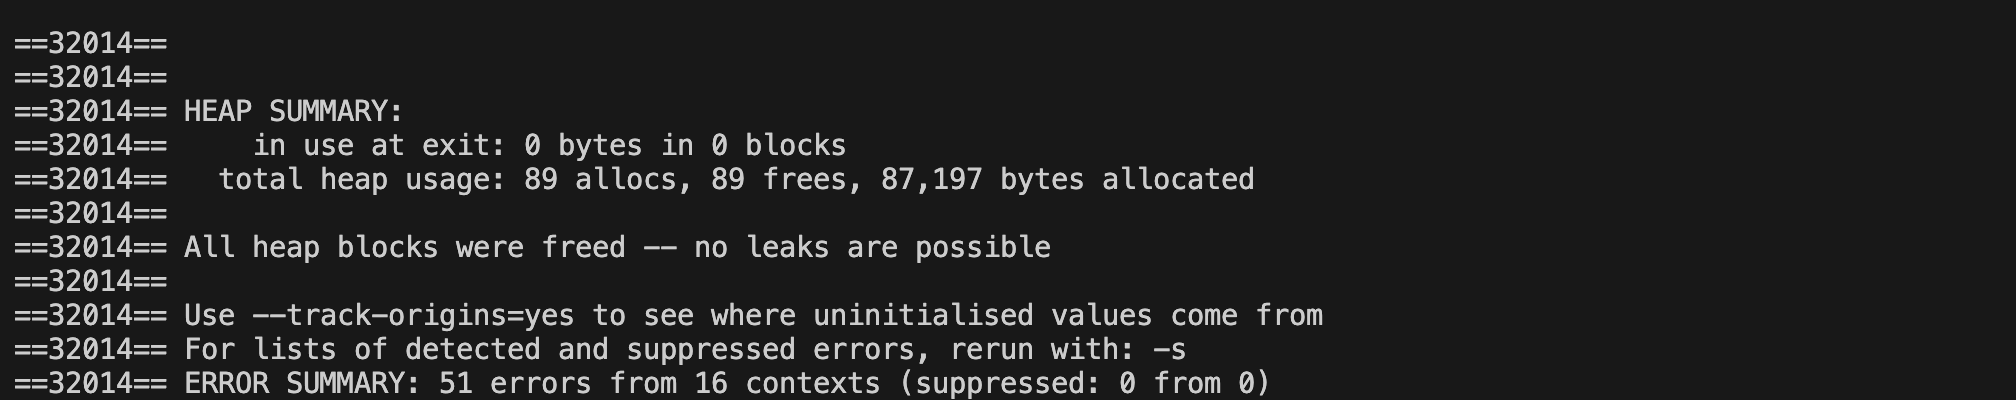
\includegraphics[width=1\textwidth]{v2.png}
    \caption{Valgrind results of TST}
    \label{fig:TST_valgrind}
\end{figure}

\section{Recurrence Analysis for TST}

\subsection{Insert Function (insert)}
\[
T(n) = T(n - 1) + O(1)
\]
Using substitution:
\[
T(n) = O(n + len(longest word))
\]
\textbf{Explanation:} The insertion can happen after traversing the longest word.

\subsection{Print Function (print)}
\[
T(n) = T(n - 1) + O(1)
\]
Using substitution:
\[
T(n) = O(n )
\]
\textbf{Explanation:} The \texttt{print} function visits each node exactly once during traversal.


\subsection{Delete Function (delete)}
\[
T(n) = T(n - 1) + O(1)
\]
Using substitution:
\[
T(n) = O(n)
\]
\textbf{Explanation:} Each node is visited and deleted exactly once.




\end{document}
